\documentclass{beamer}
%\usetheme{Madrid}
\usecolortheme{rose}
%\usefonttheme{serif}
\usepackage[utf8]{inputenc}
\usepackage[spanish]{babel}
\usepackage{graphicx}
\usepackage{amsmath} % Paquete para ecuaciones

\title{Sistema de Navegación Adaptativa para un Vehículo Autónomo}
\author{
    Over Alexander Mejia Rosado \\
    Ronald Mateo Ceballos Lozano \\
    Rhonald José Torres Díaz
}
\institute{\textit{Inteligencia Artificial} \\
Universidad Nacional de Colombia - De La Paz}
\date{}

\begin{document}

\begin{frame}
    \titlepage
\end{frame}

\begin{frame}{Introducción}
    \begin{itemize}
        \item Desarrollo de un vehículo autónomo capaz de desplazarse en un mapa 2D.
        \item Implementación del algoritmo NEAT (NeuroEvolution of Augmenting Topologies).
        \item Uso de sensores virtuales para la percepción del entorno.
        \item Aplicación de métricas de distancia (Euclidiana, Manhattan, Chebyshev) como sistema de recompensas.
        \item Creación de un sistema de refuerzo para evitar el estancamiento del vehículo.
    \end{itemize}
\end{frame}

\begin{frame}{Objetivo del Proyecto}
    \begin{itemize}
        \item Determinar que metricas de distancia son mas efectivas para el cálculo del fitness.
        \item Utilizar NEAT (NeuroEvolution of Augmenting Topologies) para desarrollar el sistema de navegación.
        \item Mejorar la capacidad del vehículo de adaptarse al entorno.
    \end{itemize}
\end{frame}

\section{Metodología}

\begin{frame}{Metodología}
    \begin{itemize}
        \item Creación del entorno 2D con la herramienta Pygame Python.
        \item Uso de métricas de distancia (Euclidiana, Manhattan, Chebyshev) como sistema de recompensas.
        \item Creación de un sistema de un metodo para evitar que el vehículo se estanque.
    \end{itemize}
\end{frame}

\begin{frame}{Entorno 2D}
    \begin{columns}
        \begin{column}{0.5\textwidth}
            \begin{figure}
                \centering
                % Primera imagen (dentro del directorio actual)
                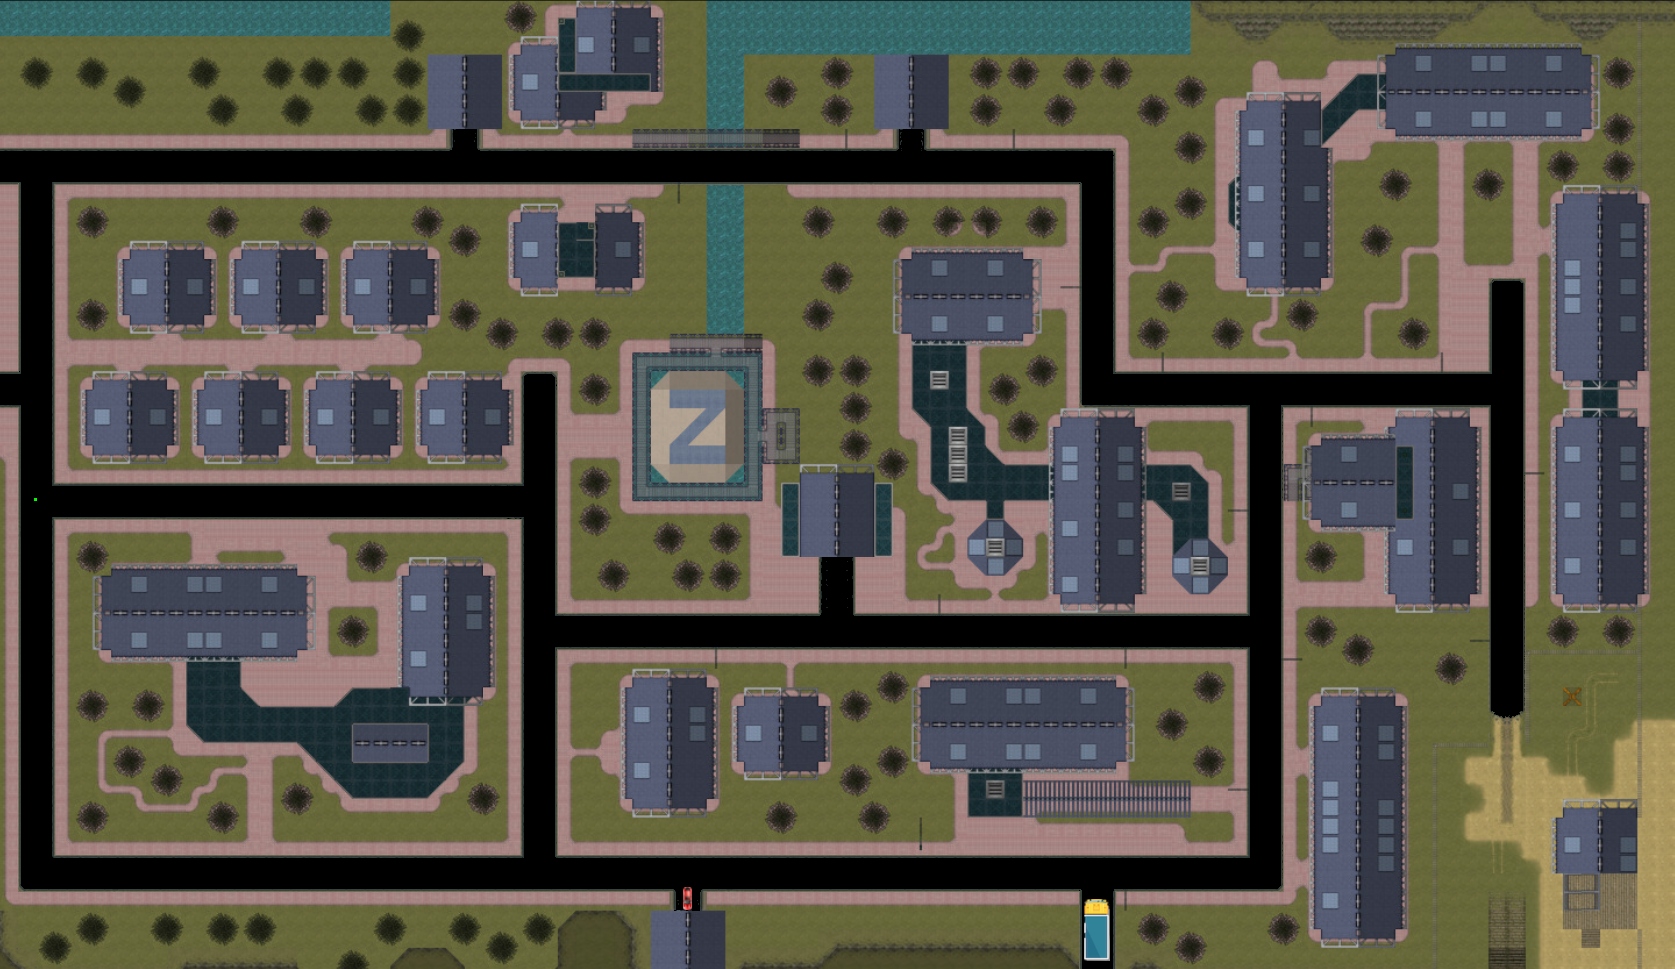
\includegraphics[width=\linewidth]{images/gta2.png}
            \end{figure}
            \vspace{0.5cm} % Espacio entre las imágenes
            \begin{figure}
                \centering
                % Segunda imagen (una carpeta atrás)
                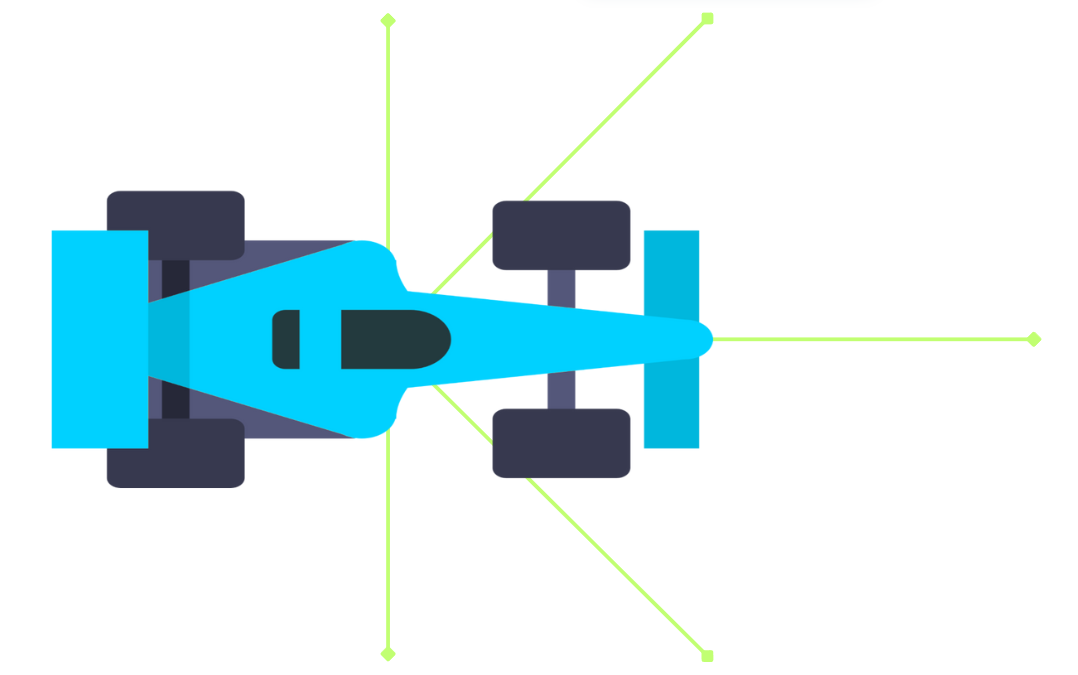
\includegraphics[width=\linewidth]{images/sensores.png}
            \end{figure}
        \end{column}
        \begin{column}{0.5\textwidth}
            \begin{itemize}
                \item Mapa 2D implementado en las simulaciones realizadas.
                \item Aplicacion de radares al agente.
                \item Angulos del los radares: -90°, -45°, 0°, 45°, 90°.
                \item Los sensores proporcionan información sobre el entorno inmediato del vehículo, incluyendo obstáculos y límites de la vía.
            \end{itemize}            
        \end{column}
    \end{columns}
\end{frame}

\begin{frame}{Metodología - Cálculo del Fitness}
\textbf{Algoritmo NEAT}
    Se utiliza NEAT para evolucionar la arquitectura de la red neuronal que controla el vehículo. NEAT permite:
\begin{itemize}
    \item Incrementar complejidad de la red gradualmente.
    \item Preservar estructuras efectivas a través de la especiación.
    \item Entre mayor sea el fitnes de un agente, aumenta la probabilidad de ser preservado para la siguiente generación.
\end{itemize}
Implementación de diferentes métricas de distancia para calcular el fitness del vehículo autónomo. La función de fitness se define como:
\begin{align*}
    \text{Fitness} = \max\left(0,\  10000 - d \right)
\end{align*}

Donde \( d \) es la distancia calculada según la métrica utilizada.

\end{frame}

\begin{frame}{Metodología - Métricas de Distancia}
  \begin{itemize}
    \item \textbf{Distancia de Manhattan}:
  \begin{align*}
    d_{\text{M}} = |x_{\text{meta}} - x_{\text{veh}}| + |y_{\text{meta}} - y_{\text{veh}}|
  \end{align*}
  
    \item \textbf{Distancia de Chebyshev}:
    \begin{align*}
        d_{\text{C}} = \max\left( |x_{\text{meta}} - x_{\text{veh}}|,\  |y_{\text{meta}} - y_{\text{veh}}| \right)
    \end{align*}

    \item \textbf{Distancia Euclidiana}:
    \begin{align*}
        d_{\text{E}} = \sqrt{(x_{\text{meta}} - x_{\text{veh}})^2 + (y_{\text{meta}} - y_{\text{veh}})^2}    
    \end{align*}

  \end{itemize}
\end{frame}

\begin{frame}{Metodología - Método Refuerzo Forzado o de Aceleración}
    \begin{columns}[T] % La opción [T] alinea el contenido en la parte superior
        \begin{column}{0.4\textwidth} % Ajusta el ancho según tus necesidades
            \begin{figure}
                \centering
                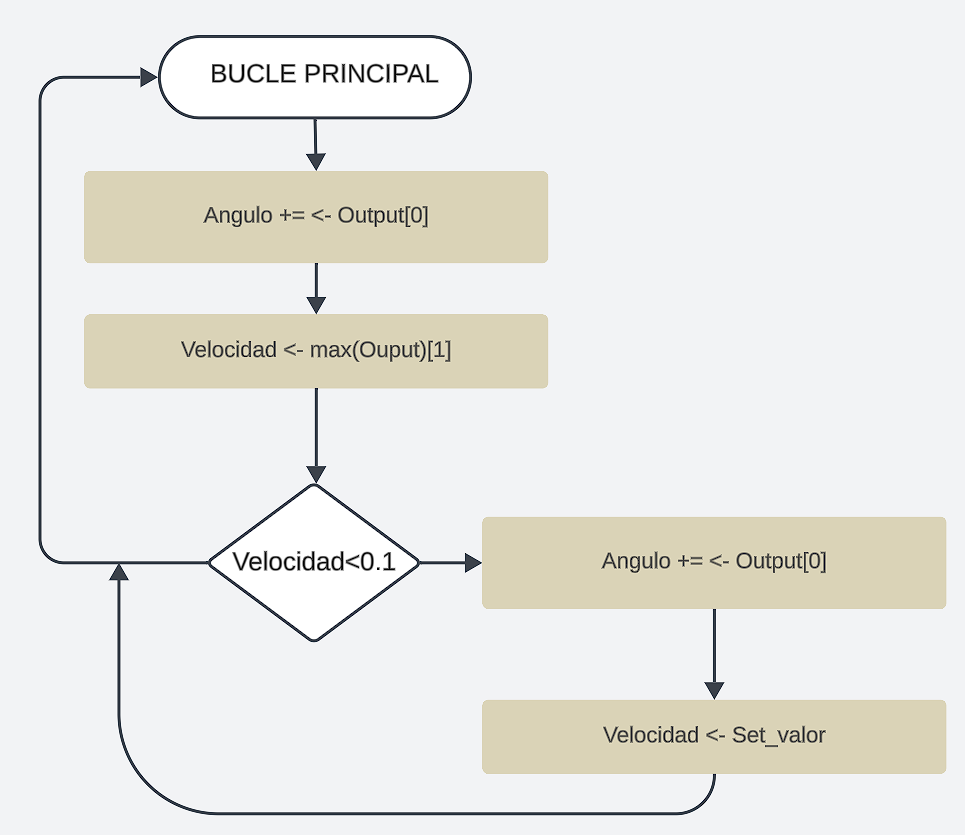
\includegraphics[width=1.1\linewidth]{images/reforce.png} % Reemplaza con la ruta correcta de tu imagen
                \caption{Esquema del Método de Refuerzo Forzado}
            \end{figure}
        \end{column}
        \begin{column}{0.6\textwidth}
            \textbf{Refuerzo Forzado}:
            \begin{itemize}
                \item Si la velocidad del vehículo es inferior a un umbral, se aplica un impulso para mantener el movimiento.
                \item Evita que el vehículo se estanque en el mapa.
            \end{itemize}
        \end{column}
    \end{columns}
\end{frame}

% Diapositiva 1: Desplazamiento Autónomo
\begin{frame}{Resultados - Desplazamiento Autónomo}
    \begin{columns}[T] % Alinea el contenido en la parte superior
        \begin{column}{0.6\textwidth}
            \begin{itemize}
                \item El vehículo autónomo logró desplazarse de manera efectiva en el mapa 2D.
                \item Capacidad de identificar y girar en las esquinas.
                \item Incremento del fitnes a lo largo de las generaciones.
            \end{itemize}
        \end{column}
        \begin{column}{0.5\textwidth}
            \begin{figure}
                \centering
                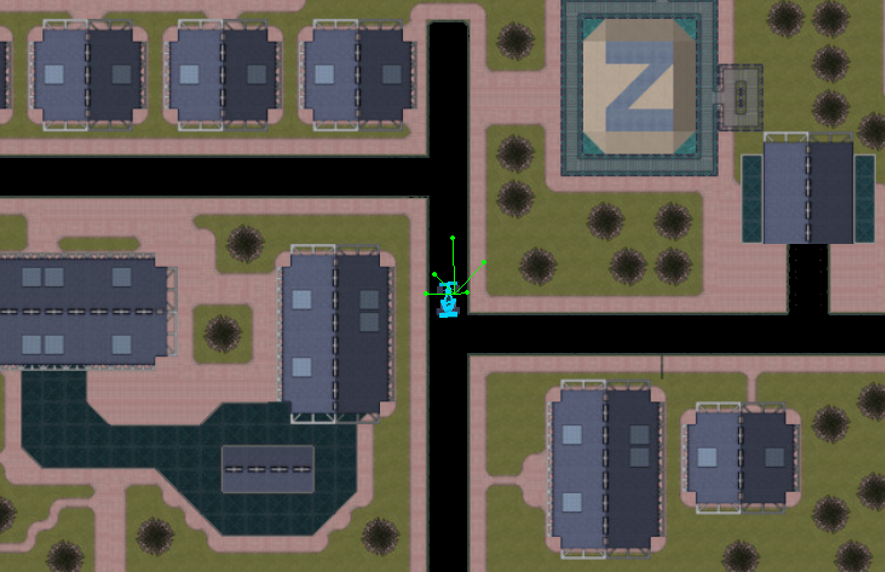
\includegraphics[width=\linewidth]{images/desplazamiento.png} % Reemplaza con la ruta correcta de tu imagen
                \caption{Vehículo autónomo en desplazamiento.}
            \end{figure}
        \end{column}
    \end{columns}
\end{frame}

% Diapositiva 2: Incremento del Fitness
\begin{frame}{Resultados - Distancia Euclidiana}
    \begin{columns}[T]
        \begin{column}{0.6\textwidth}
            \begin{itemize}
                \item Incremento constante del fitness en cada generación.
                \item Las métricas de distancia Euclidiana, Manhattan y Chebyshev mostraron diferentes tasas de mejora.
            \end{itemize}
            
        \end{column}
        \begin{column}{0.5\textwidth}
            \begin{figure}
                \centering
                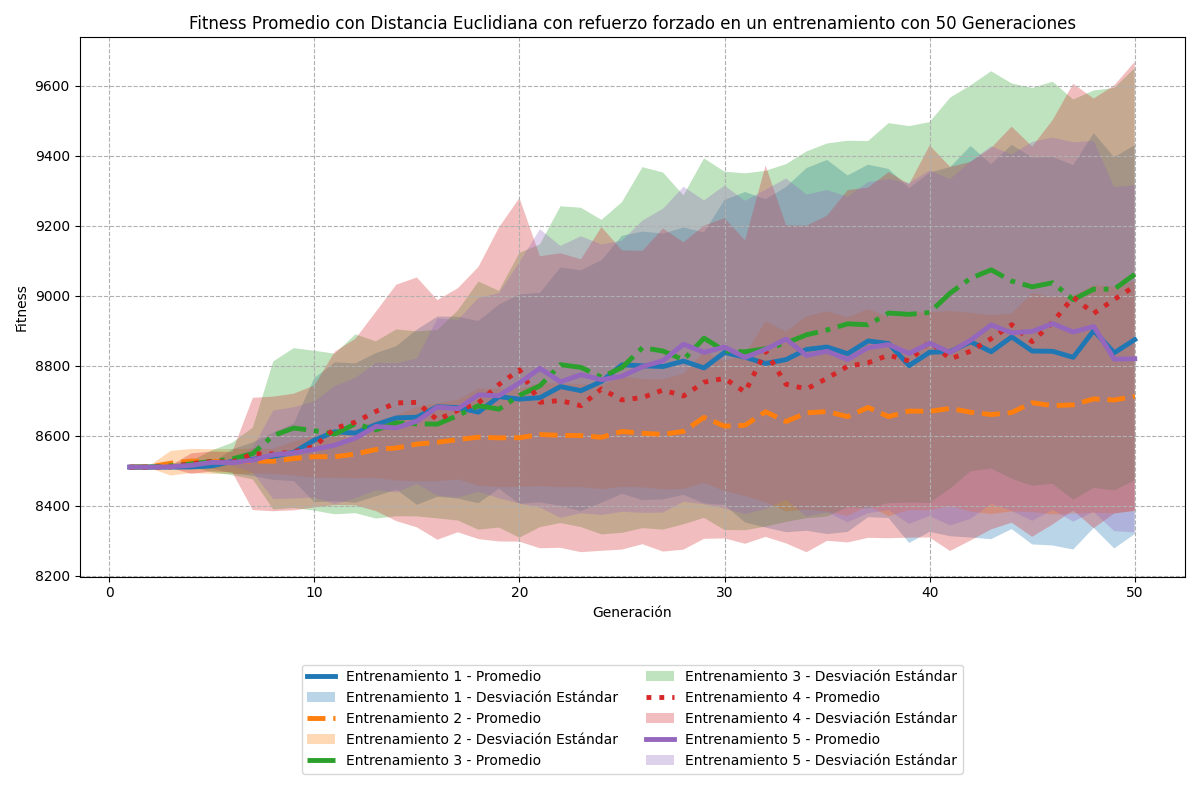
\includegraphics[width=\linewidth]{Euclidiana/Fitness_Acumulado_Eucli_50Gen.png}
                \caption{Evolución del Fitness a lo largo de las generaciones, utilizando la métrica Euclidiana.}
            \end{figure}
        \end{column}
    \end{columns}
\end{frame}



\begin{frame}{Conclusiones}
    \begin{itemize}
        \item El uso de NEAT es efectivo para desarrollar sistemas de navegación adaptativos.
        \item Las métricas de distancia y el refuerzo forzado contribuyen al aprendizaje del vehículo.
        \item Potencial para reducir accidentes y mejorar la eficiencia en sistemas de transporte autónomo.
    \end{itemize}
\end{frame}

\end{document}